  La seconde partie de notre projet à consisté à initialiser les couleurs sur les cases précédement détéctées du cube. 

  Pour cela, nous avons créé sous matlab la structure suivante : 
\begin{itemize}
  \item Cube = 6 Face ; 
  \item Face = 2 Images orientées du cube l'une colorée l'autre en niveau de gris, 1 vecteur de projection en X et 1 en Y, 9 Carre, 1 Centre, 1 Variation centre ; 
  \item Carre = 4 Points définissant une zone de calcul, 1 Centre, 1 vecteur RGB contenant la couleur moyenne calculée sur la zone caractéristique du carré ; 
  \item Centre = 1 Point ; 
  \item Point = Coordonnées (X,Y). 
\end{itemize}

  Pour initialiser nos algorithmes de reconnaissance de couleur, nous nous sommes servi des informations extraites de chacun des 6 centres des faces du cube. 
  En effet, nous savons que chaque centre est caractéristique d'un ensemble de 9 carrés d'une même couleur. 

  Nous allons donc faire de la classification pour mettre en valeur 6 groupes de 9 carrés en utilisant les valeurs RGB comme caractéristiques. 
  Nous utilisons la valeur moyenne des valeurs RGB sur une zone représentative du carré dont le centre est trouvé grâce à la méthode de la détection de contour. 

  La figure~\ref{fig:RGB_init} est celle des valeurs RGB des différents carrés, centres inclus. 
  \begin{figure}[!ht]
    \centering
    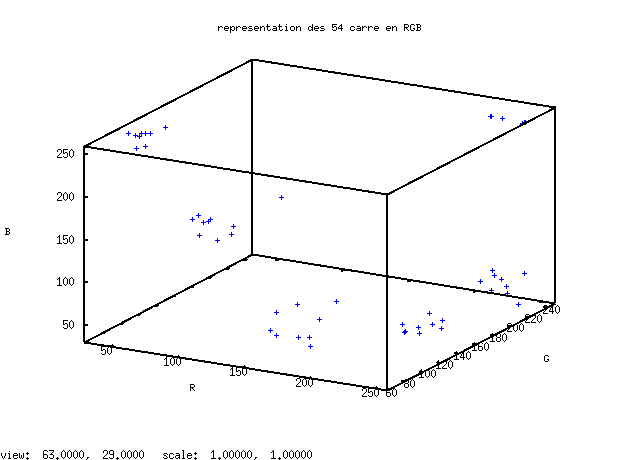
\includegraphics[width=0.5\linewidth]{./Images/RGB_init.png}
    \caption{Représentation des données RGB des différents carrés}
    \label{fig:RGB_init}
  \end{figure}

  \subsection*{Détection du centre blanc}

  Le \rubic{} que nous utilisons pour la reconnaissance a un dessin sur la face blanche, ainsi nous ne pouvons pas l'utiliser les informations de ce centre. 

  Pour détécter le centre blanc on étudie la variance des couleurs sur ces centres. 

  On obtient le résultat de la figure~\ref{fig:var} sur les 6 faces d'un même cube :
  \begin{figure}[!ht]
    \centering
    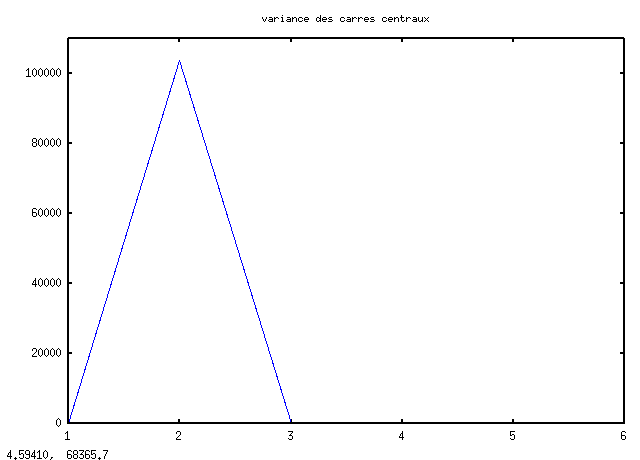
\includegraphics[width=0.5\linewidth]{./Images/var.png}
    \caption{Variance des carrés centraux}
    \label{fig:var}
   \end{figure}

  Nous pouvons constater que le centre de la face 2 a une variance beaucoup plus élevée que celle des autres. 
Ainsi nous modifions les valeurs RGB du centre mis en valeur à des valeurs correspondant à du blanc (255, 255, 255). 

  Ainsi sur des échantillons de photo prises sans reflet, on obtient avec des algorithmes tel que les K plus proches voisins (KPPV) ou le K-Means que nous avons implantés, le résultat de la figure~\ref{fig:RGBok}. 
  \begin{figure}[!ht]
    \centering
    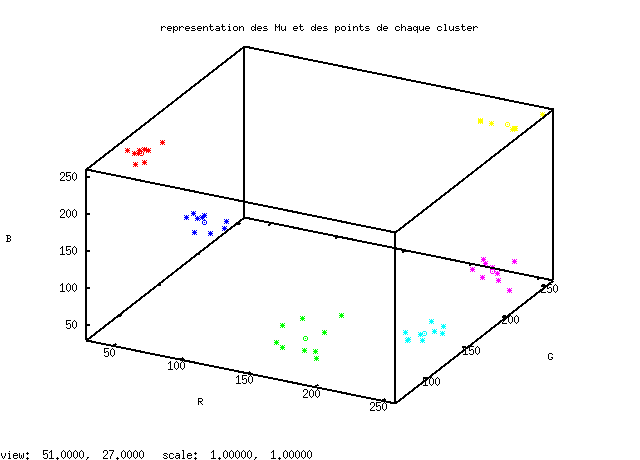
\includegraphics[width=0.5\linewidth]{./Images/RGB_ok.png}
    \caption{Variance des carrés centraux}
    \label{fig:RGBok}
   \end{figure}

  Nous obtenons bien 6 classes de 9 éléments. 
